% Copyright (c) 2015 Benito Palacios Sánchez - All Rights Reserved.
% Esta obra está licenciada bajo la Licencia Creative Commons Atribución 4.0
% Internacional. Para ver una copia de esta licencia, visita
% http://creativecommons.org/licenses/by/4.0/.

\section[Fan-traducciones]{Traducciones no oficiales}
\subsection{Saga Pokémon}

\begin{frame}{Traducciones no oficiales y Pokémon}
\pause
\note<1>[item]{Puesto el contexto sobre las ediciones de videojuegos, se va a pasar a explicar los resultados del estudio de la problemática identificada: las traducciones no oficiales, donde el caso más claro se da con la Saga Pokémon.}

\begin{columns}
  \begin{column}{0.6\textwidth}
    \begin{wideitemize}
        \item<+-> Franquicia de \textit{The Pokémon Company} fundada en 1995.
        Juegos desarrollados por \textit{Game Freak}.
        \note<1>[item]{Se fundó en 1995 por Satoshi Tajiri cuando diseñaba muñecos para la empresa Creatures Inc.}
        \note<1>[item]{El primer juego en 1996 rojo y verde, al año un millón de copias.}
        \note<1>[item]{Exclusivos de Nintendo. A día de hoy cuenta con merchandaising, ropa, cartas, películas, anime, manga, etc.}

        \item<+-> Segunda franquicia más exitosa a nivel mundial.
        \note<1>[item]{Solo está detras de Mario de Nintendo.}
        \note<1>[item]{En 2010 se llegaron a los 200 millones de copias vendidas. Solo la marca ganó en 2014 \$2.000 millones}

        \item<+-> Nº seguidores + retrasos en lanzamientos $\Rightarrow$ traducción no oficial.
        \note<1>[item]{Desde la salida de japón a América son 6 meses y a Europa otros 4.}
        \note<1>[item]{Traducciones dinámicas, parches cada semana, que quitan mercado.}
    \end{wideitemize}

    \note<1>{Se analizará la seguridad de 4 de los 6 videojuegos de esta saga. Se verá la evolución de la seguridad.}
  \end{column}

  \begin{column}{0.4\textwidth}
    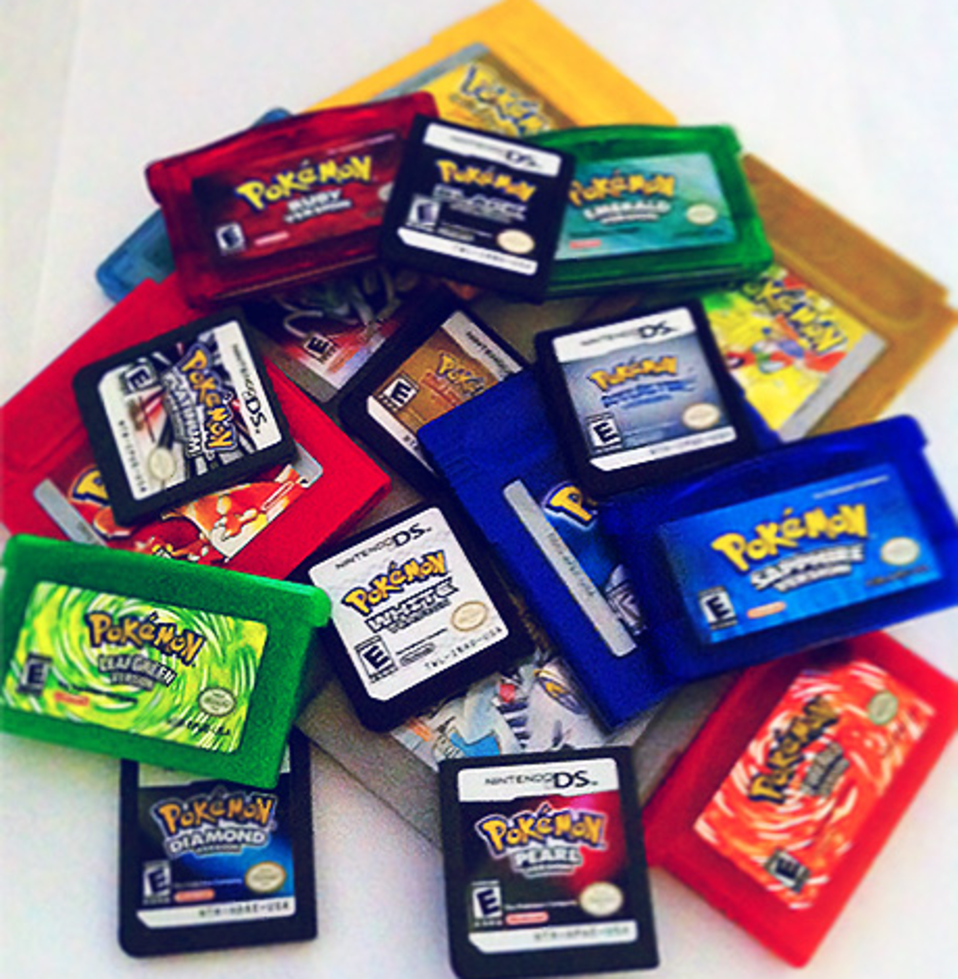
\includegraphics[width=\textwidth]{imgs/pokemon_cart.pdf}
  \end{column}
\end{columns}

\end{frame}


\begin{frame}{Metodología}

\end{frame}

\begin{frame}{Pokémon Perla y Diamante}

\end{frame}

\begin{frame}{Pokémon Blanco y Negro}

\end{frame}

\subsection{}
\begin{frame}{Mecanismos en otros juegos}
Algoritmos de protección encontrados en otros juegos:

\begin{wideitemize}
    \item<+-> \textit{Pokémon HeartGold y SoulSilver}: Igual que \textit{Pokémon Perla y Diamante}.

    \item<+-> \textit{Pokémon Conquest}: Cifra y codifica textos. Imágenes con formatos no estándar.

    \item <+-> \textit{Ninokuni - El Mago de las Tinieblas}: Cifra estadísticas de personajes y monstruos. Añade algoritmos de integridad en el archivo de guardado.
\end{wideitemize}
\end{frame}
